\documentclass{article}

% Environment setup

\usepackage[
    margin=1in
]{geometry} %geometry (sets margin) and other useful packages 
\setlength{\oddsidemargin}{.25in}
\setlength{\evensidemargin}{.25in}
\setlength{\textwidth}{6in}
\setlength{\topmargin}{-0.4in}
\setlength{\textheight}{8.5in}
\setlength{\parindent}{0em}
\setlength{\parskip}{.75em}

\usepackage{graphicx}
\usepackage{grffile}  % support extra dots in filenames
\usepackage{fancyref}
\usepackage[labelfont=bf]{caption}
\usepackage{subcaption}


\title{\textbf{CS 4641:} Supervised Learning}
\author{Bradley Reardon}
\date{February 10, 2019}

\begin{document}
    \maketitle

    \section{Introduction}
    The purpose of this assignment is to evaluate various supervised learning techniques in the context of two classification algorithms. We will focus on analyzing and adjusting five learning algorithms using two publically available data sets, through cross-validation and hyper parameter adjustments. Then, we can use our adjusted models to compare supervised learning techniques in the context of each of our classification algorithms.

    \subsection{Collaboration disclosure}
    I collaborated on planning and tuning the programming portion of this assignment with Nikolai Vorobiev in order to produce a code-base capable of using scikit-learn to effectively evaluate the given data sets. Though the code we used to run analysis on the algorithms is the same, this analysis is wholly my own.

    \section{Classification algorithms}
    For the purposes of this report, data sets were obtained from the UCI Machine Learning Repository. Each data set downloaded was processed with a custom script in the corresponding folder, \textbf{process.py}, which randomly separated the data into an 80\% training data and 20\% test data split using the \textbf{train\_test\_split} function from scikit-learn. The split data was then serialized using Python's \textbf{pickle} module into \textbf{.dataset} files, to ensure that the training and test sets remained constant for evaluation.

    For the purposes of this assignment, cross-validation scoring of the various algorithms for each classification problem will be shown as the average score of 5-fold cross validation.

    \subsection{Car data set}
    The Car Evaluation Database was created in June, 1997 by Marko Bohanec. It contains 1728 instances and six attributes. The purpose of this database is to attempt to classify a car as an unacceptable, acceptable, good, or very good choice based on factors including cost of ownership, comfort, and safety. Full details about the data set can be found at the source link below.

    The problem at hand for this data set is determining the acceptability for a car purchase based on the aforementioned attributes. Because this data set notes that the instances in the data set completely cover the attribute space, this data set is interesting in particular due to its usefulness in comparing the optimization of different supervised learning algorithms. Note that this specific data set contains only categorical attributes. As scikit-learn does not support non-continuous variables, a one-hot encoder was used to re-encode categorical features into multiple dimensions.

    \textbf{Source:} https://archive.ics.uci.edu/ml/datasets/car+evaluation

    \subsection{Breast Cancer Wisconsin data set}
    The Breast Cancer Wisconsin data set was donated to the UCI Machine Learning Repository in 1992, and contains data from one doctor's clinical cases, gathered from January 1989 to November 1991. In total, there are 699 instances signifying information about breast tumors such as clump thickness, uniformity in shape and size, and other screening factors. Data points are identified by two classes -- benign or malignant. The features of the data points are encoded as 9 continuous attributes rating the screening factor from 1 to 10.

    This data set contains unknowns in the form of question marks in the data. To deal with this, missing values were imputed, calculating missing data points based on the mean of other points in the specific column of the missing attribute. 

    The problem at hand for this data set is determining whether a tumor is benign or malignant based on tumor screening characteristics identified in the data set.

    \textbf{Source:} https://archive.ics.uci.edu/ml/datasets/Breast+Cancer+Wisconsin+\%28Original\%29

    \section{Decision trees with pruning}

    \subsection{Parameter selection}
    To begin evaluating the decision tree algorithm, hyper parameter selection was essential to tuning the algorithms to each data set. Both the car and cancer data sets were evaluated with the GINI index criterion as well as the entropy criterion. The two criterion had no discernible differences in training results, so as a result, GINI was selected for the decision tree classifier on both sets, as it allows us to avoid a logarithmic calculation, saving compute time.

    The next parameters that needed tuning were the pruning parameters included in the scikit-learn decision tree classifier. Namely, the max depth of the tree, as well as the minimum samples per leaf, were tuned to fit each data set.

    For the car data set, parameter selection showed that a lower-depth tree had much lower accuracy, likely due to the fact that the data set had instances covering the entire attribute space. As a result, a max depth of 9 nodes was selected for the car data set, with a minimum number of 5 samples occurring at each leaf node to minimize the amount of information loss.

    The cancer data set, on the other hand, responded much better to more aggressive pruning. The pruned decision tree classifier responded to the data with the best F1 score with a max depth of 5 nodes, and a minimum number of 10 samples occurring at each leaf.

    \subsection{Performance}
    Performance of the tuned classifier for each data set was measured with both wall clock time for fitting the model with the training data, as well as making a prediction with the test data. For the breast cancer data set, pruning resulted in both higher precision and accuracy, with a performance gain during prediction over a non-pruned decision tree (from 0.801ms to 0.479ms). However, the classifier took 0.57ms longer to train with pruning enabled (no pruning: 2.38ms, pruning: 2.95ms). For this data set, with the determined parameters was successful.

    However, the car data set showed different results with pruning enabled. There was no significant change in either the precision or accuracy measures. The car data set's decision tree classifier took 11.51ms to fit without pruning, however with pruning this was reduced to 7.35ms with pruning. Prediction runtime for the pruned tree was only slightly longer than the unpruned tree. Due to the completeness of the data, pruning is likely not necessary for this data set without further tuning.

    Learning curves for the data sets, with and without pruning enabled, can be found in \Fref{fig:dt-learning}.

    \begin{figure}[htb]
    \centering

    \begin{subfigure}{0.5\textwidth}
      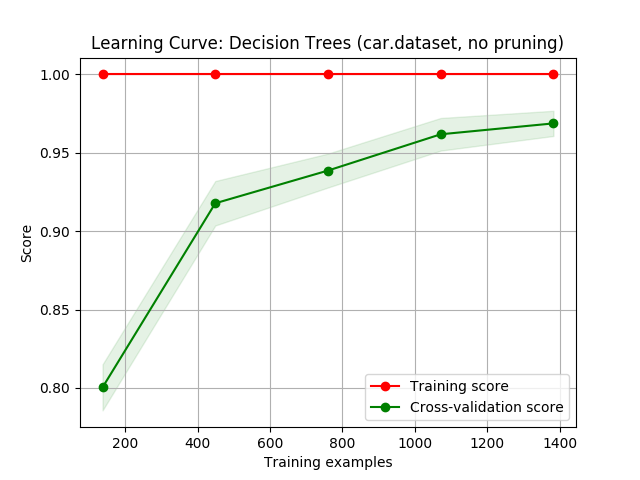
\includegraphics[width=\linewidth]{out/decision_tree_pruning/car-noprune-learning.png}
      \caption{Car data set, no pruning}
      \label{fig:dt-learning-1}
    \end{subfigure}\hfil
    \begin{subfigure}{0.5\textwidth}
      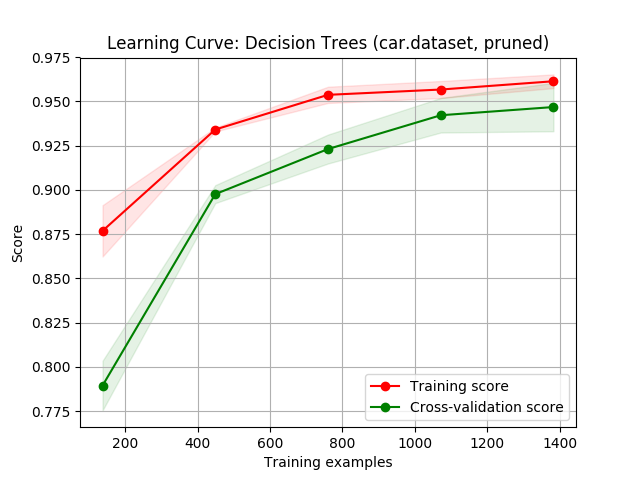
\includegraphics[width=\linewidth]{out/decision_tree_pruning/car-prune-learning.png}
      \caption{Car data set, with pruning}
      \label{fig:dt-learning-2}
    \end{subfigure}

    \medskip

    \begin{subfigure}{0.5\textwidth}
      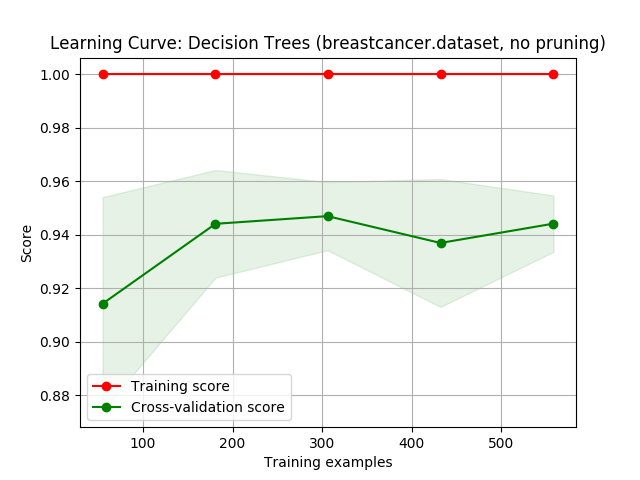
\includegraphics[width=\linewidth]{out/decision_tree_pruning/breastcancer-noprune-learning.png}
      \caption{Breast cancer data set, no pruning}
      \label{fig:dt-learning-3}
    \end{subfigure}\hfil
    \begin{subfigure}{0.5\textwidth}
      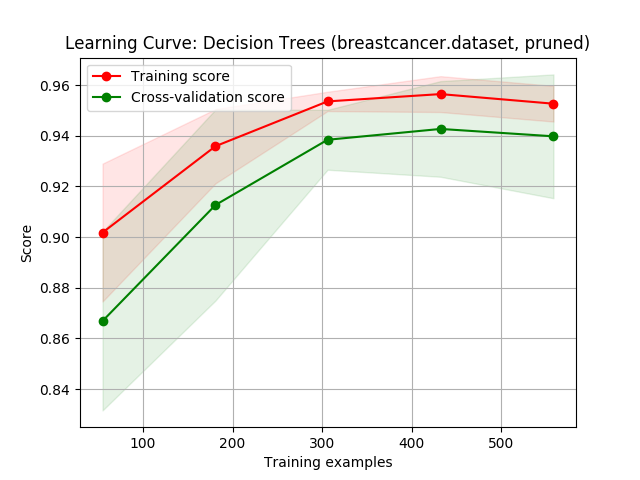
\includegraphics[width=\linewidth]{out/decision_tree_pruning/breastcancer-prune-learning.png}
      \caption{Breast cancer data set, with pruning}
      \label{fig:dt-learning-4}
    \end{subfigure}

    \caption{Learning curves for the car and breast cancer data sets using a decision tree classifier, with and without pruning.}
    \label{fig:dt-learning}
    \end{figure}

    \section{Boosting}
    We will next evaluate the AdaBoost boosting algorithm included in scikit-learn, using the pruned decision trees from the previous section as base estimators for the algorithm.

    \subsection{Parameter selection}
    For the AdaBoost algorithm, there were three main parameters that needed to be determined. The graphs in \Fref{fig:boosting-param} were used to determine the proper learning rate, number of estimators, and algorithm for both data sets.

    \begin{itemize}
        \item \textbf{n\_estimators:} the max number of classifiers (decision trees) to fit to the AdaBoost classifier
        \item \textbf{learning\_rate:} shrinks the contribution of each classifier by this amount
        \item \textbf{algorithm:} scikit-learn supports two algorithms derived from AdaBoost -- AdaBoost-SAMME and AdaBoost-SAMME.R. SAMME is usually used for discrete values, whereas SAMME.R is used for real/continuous values. 
    \end{itemize}

    The graphs in \Fref{fig:boosting-param} show that the car data generally has lower error with the SAMME algorithm, whereas the breast cancer data leads to lower error when fit with the SAMME.R algorithm. For both sets, the error was generally minimized with a learning rate of 1.0, so that rate was selected for both classifiers.

    \begin{figure}[htb]
    \centering

    \begin{subfigure}{0.33\textwidth}
      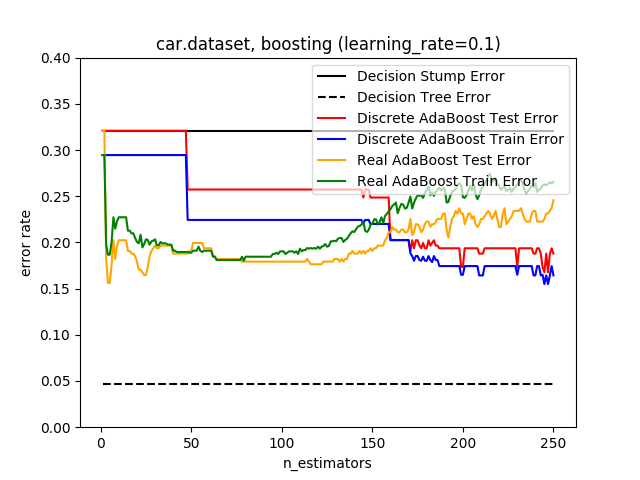
\includegraphics[width=\linewidth]{out/boosting/car-error-lrate-0.1.png}
      \caption{Car data, l\_rate=0.1}
      \label{fig:boosting-param-1}
    \end{subfigure}\hfil
    \begin{subfigure}{0.33\textwidth}
      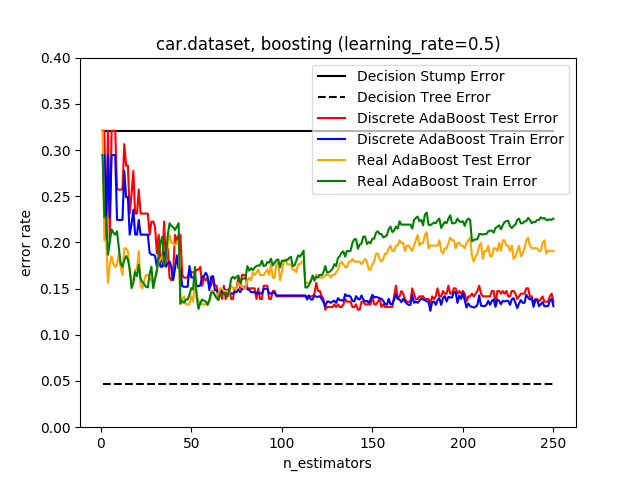
\includegraphics[width=\linewidth]{out/boosting/car-error-lrate-0.5.png}
      \caption{Car data, l\_rate=0.5}
      \label{fig:boosting-param-2}
    \end{subfigure}\hfil
    \begin{subfigure}{0.33\textwidth}
      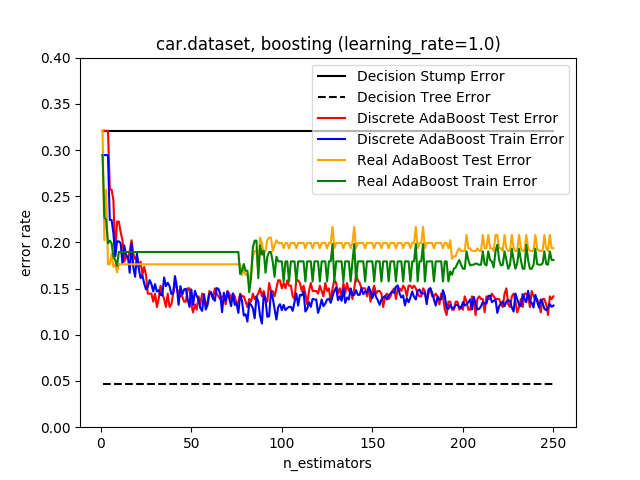
\includegraphics[width=\linewidth]{out/boosting/car-error-lrate-1.0.png}
      \caption{Car data, l\_rate=1.0}
      \label{fig:boosting-param-3}
    \end{subfigure}

    \medskip

    \begin{subfigure}{0.33\textwidth}
      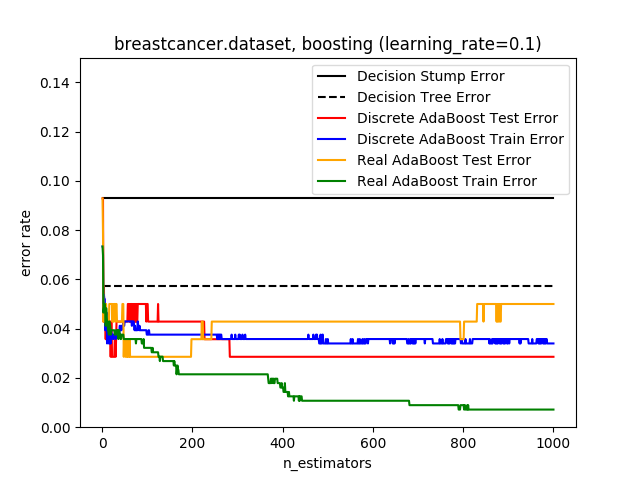
\includegraphics[width=\linewidth]{out/boosting/breastcancer-error-lrate-0.1.png}
      \caption{Cancer data, l\_rate=0.1}
      \label{fig:boosting-param-4}
    \end{subfigure}\hfil
    \begin{subfigure}{0.33\textwidth}
      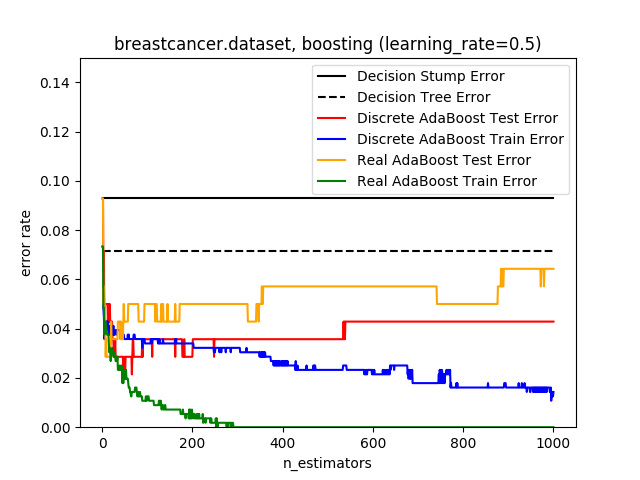
\includegraphics[width=\linewidth]{out/boosting/breastcancer-error-lrate-0.5.png}
      \caption{Cancer data, l\_rate=0.5}
      \label{fig:boosting-param-5}
    \end{subfigure}\hfil
    \begin{subfigure}{0.33\textwidth}
      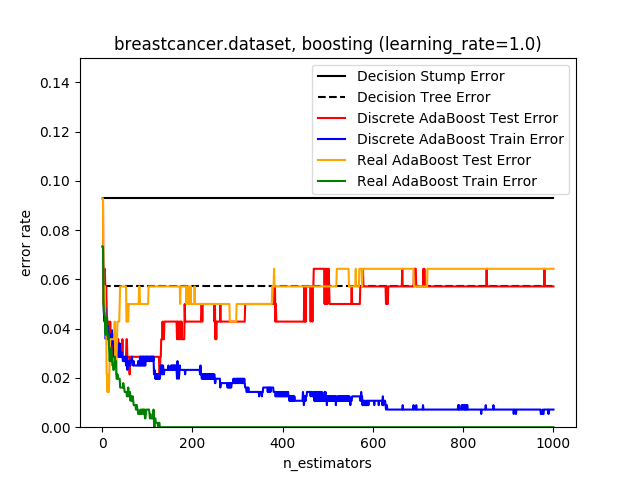
\includegraphics[width=\linewidth]{out/boosting/breastcancer-error-lrate-1.0.png}
      \caption{Cancer data, l\_rate=1.0}
      \label{fig:boosting-param-6}
    \end{subfigure}

    \caption{Selecting a learning rate and number of estimators for the AdaBoot algorithm, using the car and breast cancer sets.}
    \label{fig:boosting-param}
    \end{figure}

    The number of estimators was also determined from the error graphs in \Fref{fig:boosting-param}. The lowest number of estimators where error for the chosen algorithm was minimized was chosen as the number of estimators for each data set. For the car data set, this was approximately 100 estimators, while the cancer data set performed best with around 200 estimators.

    \subsection{Performance}
    \Fref{fig:boosting-perf} shows the learning curves for the car and data set pruned decision tree classifiers before and after applying boosting. Boosting provided a tangible benefit in accuracy and precision for both data sets after proper parameter selection. With the chosen parameters, the car data set and the cancer data set both showed better cross-validation scores with boosting than over the standard pruned decision tree classifiers in the previous section.

    \begin{figure}[htb]
    \centering

    \begin{subfigure}{0.5\textwidth}
      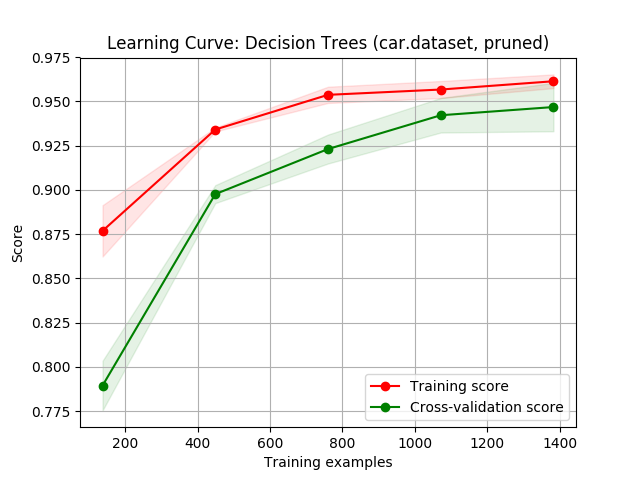
\includegraphics[width=\linewidth]{out/decision_tree_pruning/car-prune-learning.png}
      \caption{Car data, pruning, no boosting}
      \label{fig:boosting-perf-1}
    \end{subfigure}\hfil
    \begin{subfigure}{0.5\textwidth}
      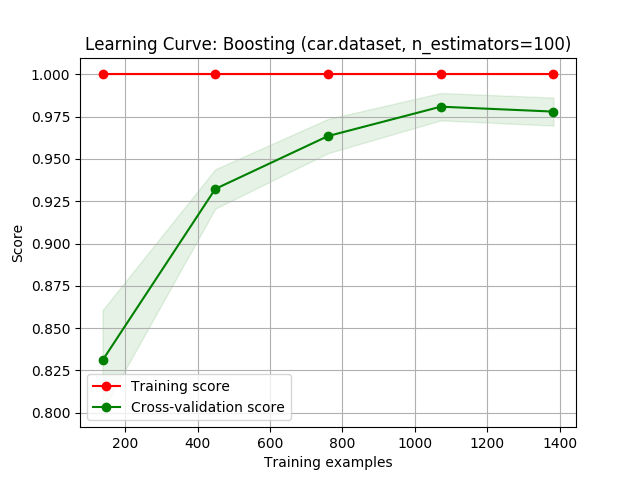
\includegraphics[width=\linewidth]{out/boosting/car-estimators-100.png}
      \caption{Car data, pruning, with boosting}
      \label{fig:boosting-perf-2}
    \end{subfigure}

    \medskip

    \begin{subfigure}{0.5\textwidth}
      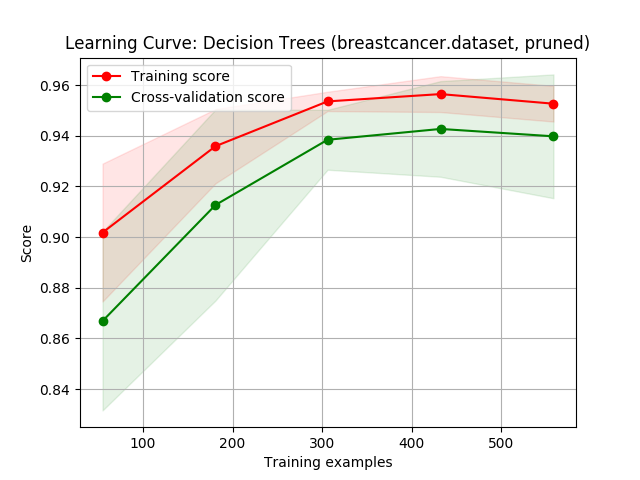
\includegraphics[width=\linewidth]{out/decision_tree_pruning/breastcancer-prune-learning.png}
      \caption{Breast cancer data, pruning, no boosting}
      \label{fig:boosting-perf-3}
    \end{subfigure}\hfil
    \begin{subfigure}{0.5\textwidth}
      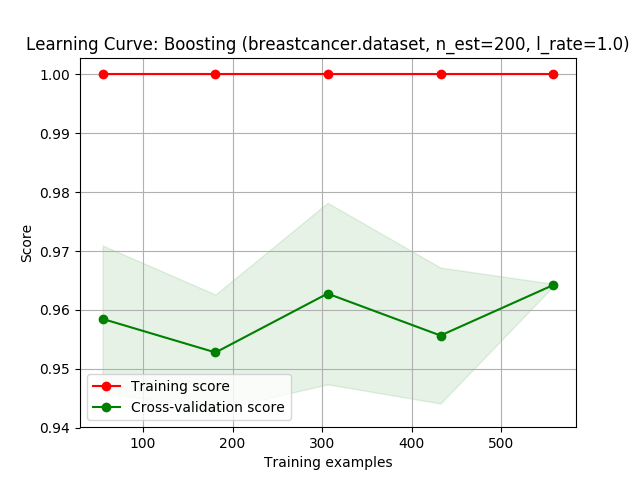
\includegraphics[width=\linewidth]{out/boosting/breastcancer-estimators-200.png}
      \caption{Breast cancer data, pruning, with boosting}
      \label{fig:boosting-perf-4}
    \end{subfigure}

    \caption{Learning curves for the car and cancer data sets, with and without boosting on a pruned decision tree.}
    \label{fig:boosting-perf}
    \end{figure}

    However, this increase in accuracy and precision for both data sets does come at the cost of extra wall clock time during both the fit and predict phases of testing. Due to the nature of the AdaBoost algorithm, fit and prediction times increase with some linearity to the number of estimators used to fit the classifier. This increase in time represented approximate 70-fold and 61-fold increases in fit times for the cancer and car data sets respectively. Similar slow downs resulted in prediction using the boosting algorithm over a standard pruned decision tree.

    Therefore, boosting does increase the accuracy and precision for both models, however at the cost of slowing down fit and classification times across the board. This tradeoff will be discussed further in a later section.

    \section{$k$-nearest neighbors}
    Next, the $k$-nearest neighbors algorithm was tuned and evaluated for performance on the two data sets.

    \subsection{Parameter selection}
    The main parameter adjustment for the $k$-nearest neighbors algorithm was setting a sensible value for $k$ such that cross-validation score is maximized. \Fref{fig:knn-param} shows the performance of the algorithm for each data set, with different values of $k$.

    \begin{figure}[htb]
    \centering

    \begin{subfigure}{0.5\textwidth}
      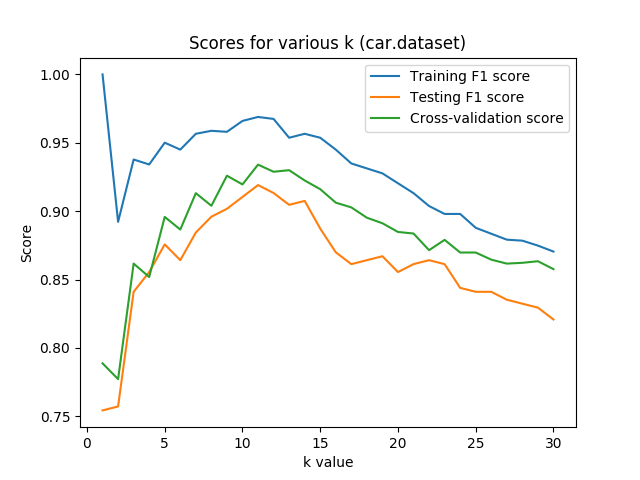
\includegraphics[width=\linewidth]{out/knn/car-k-testing.png}
      \caption{Car data set}
      \label{fig:knn-param-1}
    \end{subfigure}\hfil
    \begin{subfigure}{0.5\textwidth}
      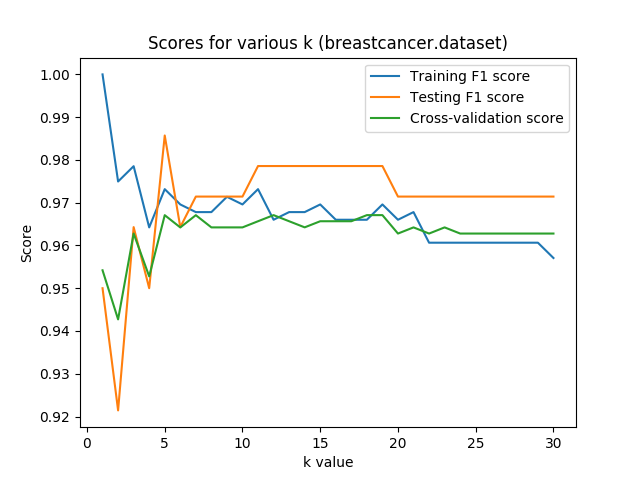
\includegraphics[width=\linewidth]{out/knn/breastcancer-k-testing.png}
      \caption{Breast cancer data set}
      \label{fig:knn-param-2}
    \end{subfigure}

    \caption{Testing $k$-nearest neighbors with various values of $k$.}
    \label{fig:knn-param}
    \end{figure}

    Cross-validation scores were best for the car data set with a value of $k=11$, whereas the cancer data performed best with $k=5$. Therefore, these values were selected as the optimal parameters of the data sets.

    \subsection{Performance}
    The $k$-nearest neighbors algorithm performed better for the breast cancer data set than the car data set with optimized values of $k$. This is likely due to the fact that the breast cancer data contains only continuous attributes, while the car data set contains only nominal data. The testing F1 scores for the cancer and car data sets using this algorithm were 98.57\% and 91.91\% respectively.

    In terms of wall clock performance, $k$-nearest neighbors was reasonably fast to fit the classifier to both sets, doing so in 4.97ms for the car data set and 2.17ms for the cancer data set. However, prediction time for the car data set was significantly slower than other algorithms at 23.84ms, whereas the cancer data set also had a relatively slow prediction runtime of 5.33ms.

    \Fref{fig:knn-learning} shows the learning curves for the two data sets using $k$-nearest neighbors with optimized $k$.

    \begin{figure}[htb]
    \centering

    \begin{subfigure}{0.5\textwidth}
      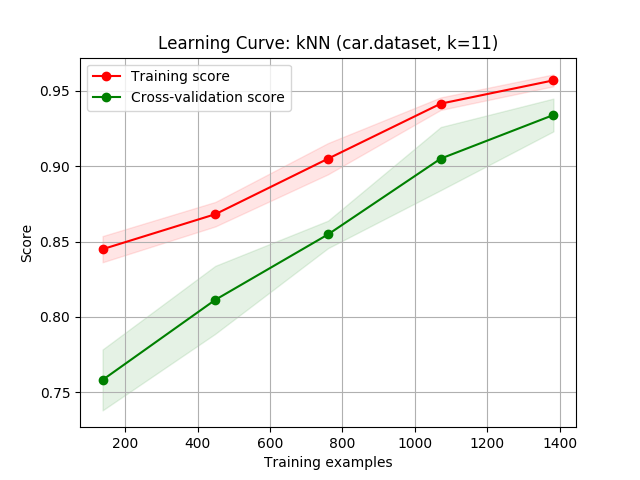
\includegraphics[width=\linewidth]{out/knn/car-k-11.png}
      \caption{Car data set, $k=11$}
      \label{fig:knn-learning-1}
    \end{subfigure}\hfil
    \begin{subfigure}{0.5\textwidth}
      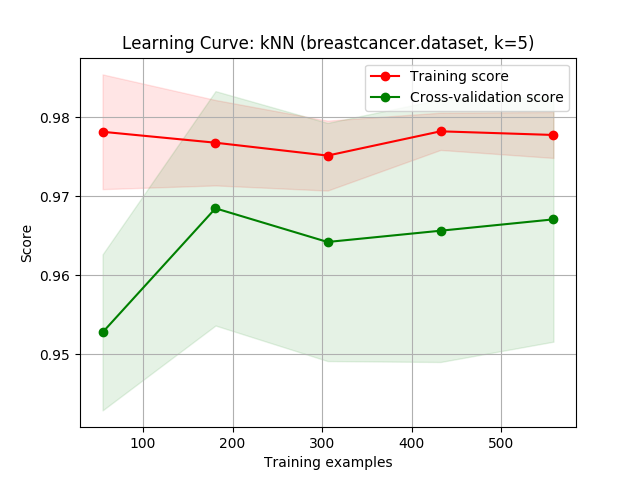
\includegraphics[width=\linewidth]{out/knn/breastcancer-k-5.png}
      \caption{Breast cancer data set, $k=5$}
      \label{fig:knn-learning-2}
    \end{subfigure}

    \caption{Learning curves for $k$-nearest neighbors with optimized $k$-values.}
    \label{fig:knn-learning}
    \end{figure}

    \section{Support vector machines}
    Support vector machines (SVMs) are the next algorithm that will be evaluated. The car and cancer data sets were both evaluated using the linear, RBF, and polynomial kernels included in scikit-learn. For the sake of brevity, the three algorithms were evaluated with otherwise default kernel parameters.

    \subsection{Kernel selection}
    Kernel selection is important for ensuring that the support vector machine is able to find the shape of the feature boundary within the attribute space. To evaluate the merits of the linear, RBF, and polynomial kernels, a learning curve was generated for each data set with each of the three kernels.

    It is immediately obvious that the polynomial kernel does not sufficiently classify the data for the car data set. This, along with the RBF kernel's reduced performance on the car data set with respect to the linear kernel, suggests that the car data set is linearly separable. Thus, the ideal kernel for the car data set is chosen to be the linear kernel.

    However, for the cancer data set, all three kernels report decent scores. The linear kernel again performs best, though the RBF kernel is close behind. The polynomial kernel also has above-90\% cross-validation score. These results suggest that, with sufficient kernel parameter tuning, a SVM trained on the cancer data set may have better accuracy than the linear kernel than with the RBF or polynomial kernels. However, for the purpose of the assignment, we select the linear kernel for use with the cancer data as well.

    The learning curves used for this evaluation can be found in \Fref{fig:svm-learning}.

    \begin{figure}[htb]
    \centering

    \begin{subfigure}{0.33\textwidth}
      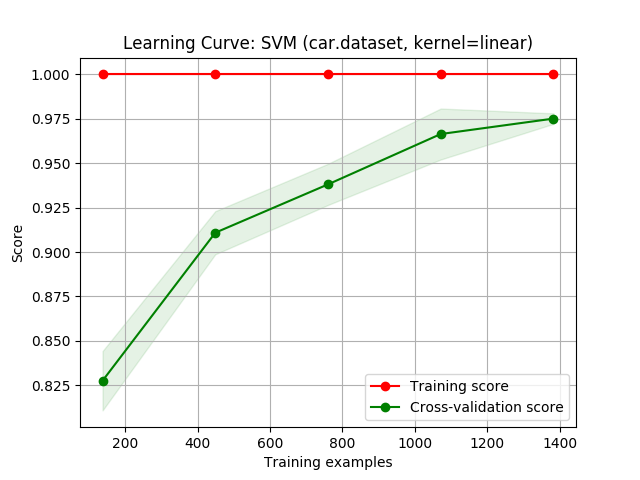
\includegraphics[width=\linewidth]{out/svm/car-kernel-linear.png}
      \caption{Car data, linear kernel}
      \label{fig:svm-learning-1}
    \end{subfigure}\hfil
    \begin{subfigure}{0.33\textwidth}
      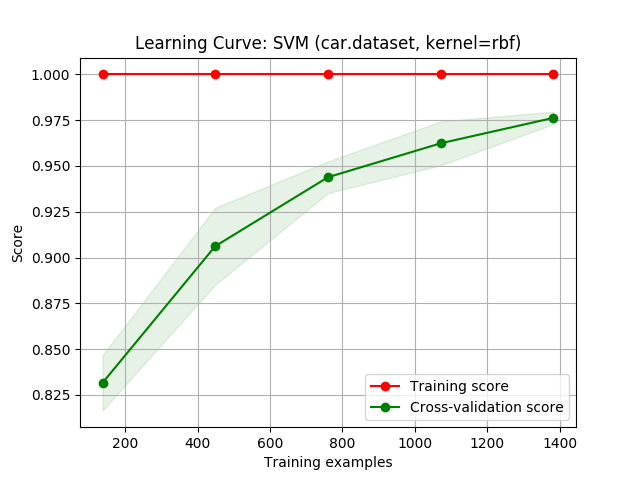
\includegraphics[width=\linewidth]{out/svm/car-kernel-rbf.png}
      \caption{Car data, RBF kernel}
      \label{fig:svm-learning-2}
    \end{subfigure}\hfil
    \begin{subfigure}{0.33\textwidth}
      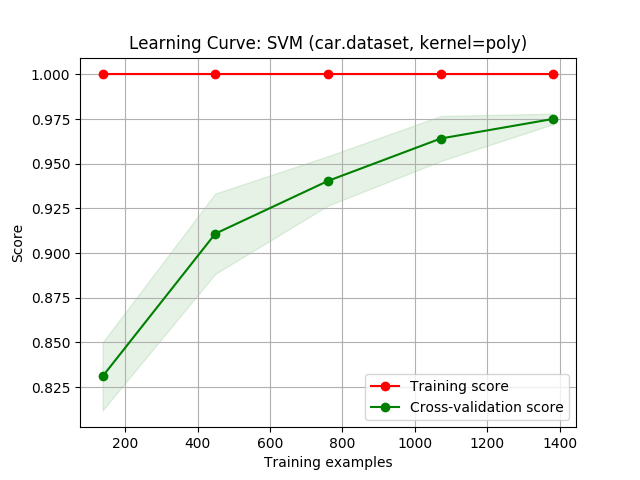
\includegraphics[width=\linewidth]{out/svm/car-kernel-poly.png}
      \caption{Car data, poly kernel}
      \label{fig:svm-learning-3}
    \end{subfigure}

    \medskip

    \begin{subfigure}{0.33\textwidth}
      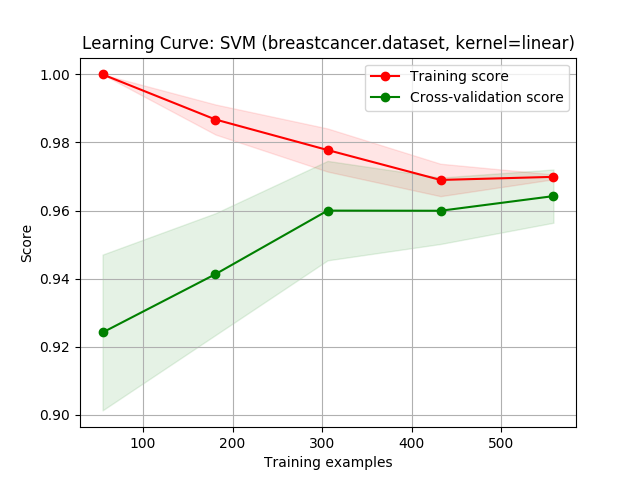
\includegraphics[width=\linewidth]{out/svm/breastcancer-kernel-linear.png}
      \caption{Breast cancer, linear kernel}
      \label{fig:svm-learning-4}
    \end{subfigure}\hfil
    \begin{subfigure}{0.33\textwidth}
      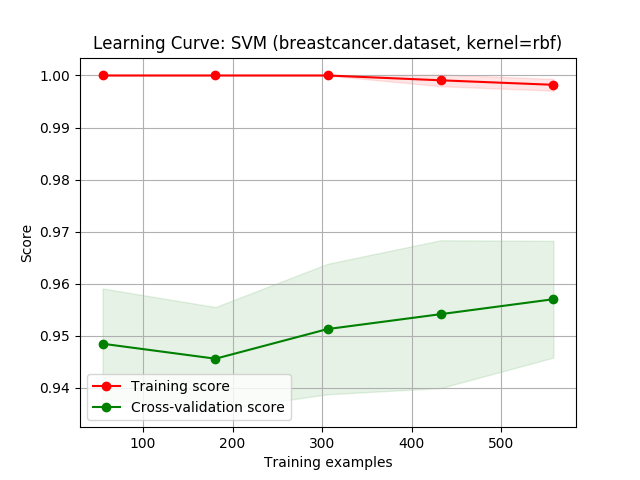
\includegraphics[width=\linewidth]{out/svm/breastcancer-kernel-rbf.png}
      \caption{Breast cancer, RBF kernel}
      \label{fig:svm-learning-5}
    \end{subfigure}\hfil
    \begin{subfigure}{0.33\textwidth}
      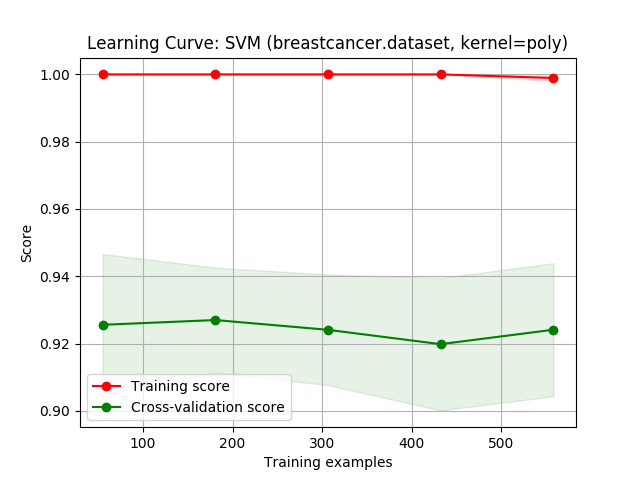
\includegraphics[width=\linewidth]{out/svm/breastcancer-kernel-poly.png}
      \caption{Breast cancer, poly kernel}
      \label{fig:svm-learning-6}
    \end{subfigure}

    \caption{Learning curves for the car and breast cancer data sets using an SVM classifier, with linear, RBF, and poly kernels.}
    \label{fig:svm-learning}
    \end{figure}

    \subsection{Performance}
    The support vector machine for the cancer data set performed well with the linear kernel. Wall clock time to fit the classifier was only 6.25ms, with a tested prediction runtime of 0.57ms. The F1 score reported for the test data was 96.43\%, indicating good accuracy for the model.

    On the other hand, the SVM trained with the car data set and the linear kernel had good, but not excellent results in terms of both accuracy and wall clock time. The test F1 score was 93.06\%, however the model took 40.81ms to fit, with a less-than-impressive prediction runtime of 6.76ms. In terms of accuracy, the car data set performed well with a linear kernel, however the wall clock time for using SVM for this data set leaves this algorithm as a less-than-desirable choice for real-world use.

    \section{Neural networks}
    Finally, we evaluate scikit-learn's built in multi-layer perceptron neural network algorithm for classifying our two data sets.

    \subsection{Solver selection}
    Because neural network generation is computationally intensive, parameter selection for the neural network algorithm was restricted to selecting the best solver for weight optimization. The three options that scikit-learn provides are the `adam' solver, the `sgd' (or stochastic gradient descent) solver, and the `lbfgs' solver. Neural networks were allowed 1,000 total iterations each to ensure the highest possibility of convergence without compromising in too much compute time.

    The learning curves used for this evaluation can be found in \Fref{fig:nn-param}.

    \begin{figure}[htb]
    \centering

    \begin{subfigure}{0.33\textwidth}
      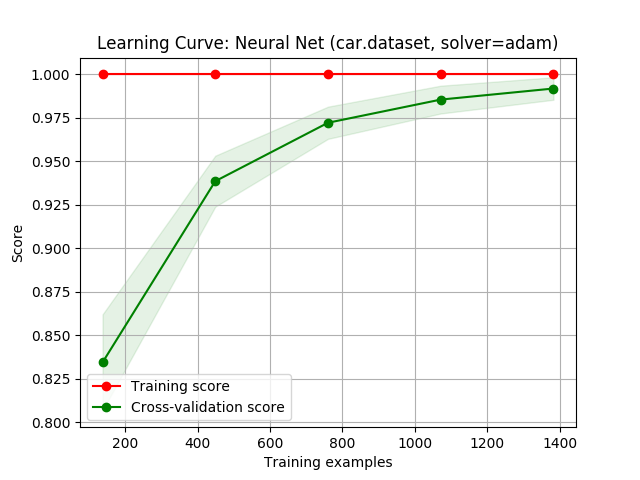
\includegraphics[width=\linewidth]{out/neural_net/car-solver-adam.png}
      \caption{Car data, adam solver}
      \label{fig:nn-param-1}
    \end{subfigure}\hfil
    \begin{subfigure}{0.33\textwidth}
      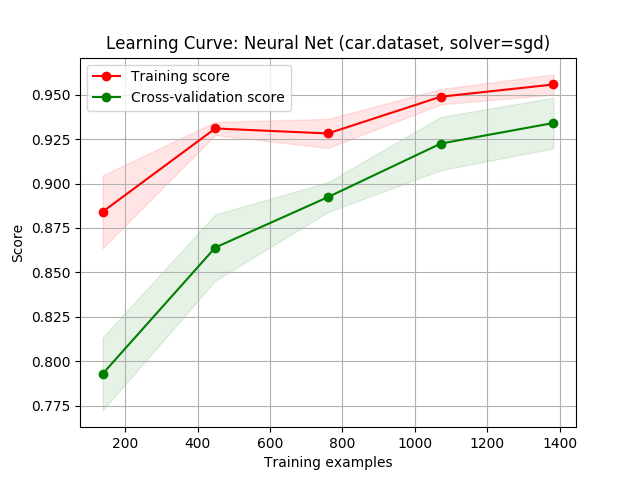
\includegraphics[width=\linewidth]{out/neural_net/car-solver-sgd.png}
      \caption{Car data, sgd solver}
      \label{fig:nn-param-2}
    \end{subfigure}\hfil
    \begin{subfigure}{0.33\textwidth}
      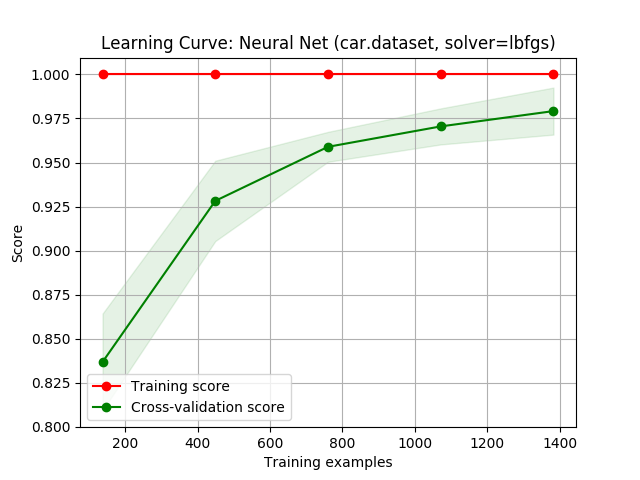
\includegraphics[width=\linewidth]{out/neural_net/car-solver-lbfgs.png}
      \caption{Car data, lbfgs solver}
      \label{fig:nn-param-3}
    \end{subfigure}

    \medskip

    \begin{subfigure}{0.33\textwidth}
      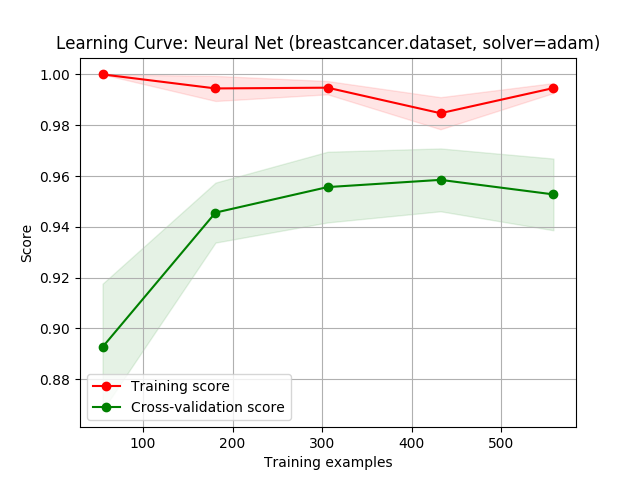
\includegraphics[width=\linewidth]{out/neural_net/breastcancer-solver-adam.png}
      \caption{Breast cancer, adam solver}
      \label{fig:nn-param-4}
    \end{subfigure}\hfil
    \begin{subfigure}{0.33\textwidth}
      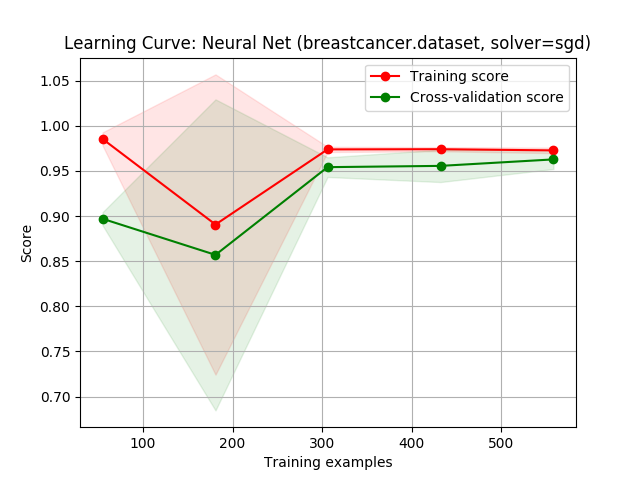
\includegraphics[width=\linewidth]{out/neural_net/breastcancer-solver-sgd.png}
      \caption{Breast cancer, sgd solver}
      \label{fig:nn-param-5}
    \end{subfigure}\hfil
    \begin{subfigure}{0.33\textwidth}
      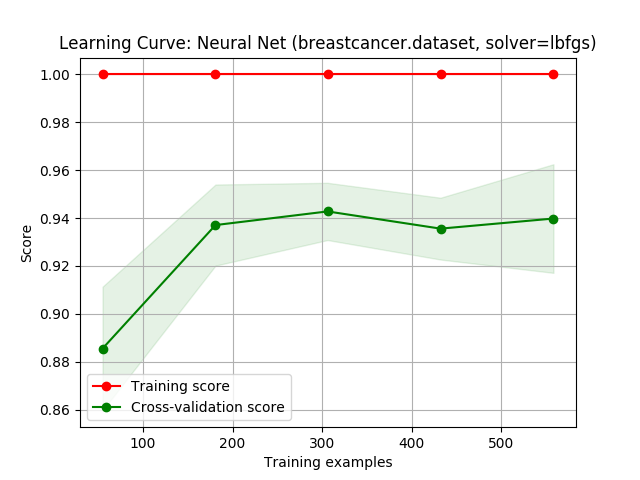
\includegraphics[width=\linewidth]{out/neural_net/breastcancer-solver-lbfgs.png}
      \caption{Breast cancer, lbfgs solver}
      \label{fig:nn-param-6}
    \end{subfigure}

    \caption{Learning curves for the car and breast cancer data sets using a MLP neural network, with adam, sgd, and lbfgs solvers.}
    \label{fig:nn-param}
    \end{figure}

    Cursory analysis of the learning curves for the different solvers shows that, for the car data set, the `adam' and `lbfgs' solvers perform very well with default parameters. On a single run, `lbfgs' performed better than the `adam' solver, however, due to the lower variance in cross-validation score of the `adam' solver, we'll further discuss this implementation using only the `adam' solver.

    The breast cancer data set, however, showed the best accuracy and lowest variance cross-validation score when using the `sgd' solver. Thus, further analysis will occur using the `sgd' solver on the breast cancer data set.

    Note that stochastic gradient descent is heavily tunable via hyper parameters, however in the interest of time, the defaults were used in all cases to get a good overview of algorithmic performance out of the box.

    \subsection{Performance}
    Neural networks can be extremely accurate, but often at the cost of model fitting time. This was very evident with neural networks in this analysis.

    The car data set's model was built in 2.33 seconds of wall clock time, which is much longer than any of the other algorithms discussed in this report. However, prediction runtime for the `adam'-solved neural network were relatively low, at 1.68ms for a single prediction. The neural network's testing F1 score was 97.69\%, indicating extremely good accuracy on unseen data.

    The breast cancer data set's neural network, generated with the `sgd' solver, fared well, but not as well as the car data's neural network. The testing F1 score of the breast cancer neural network was 94.29\%, which still indicates good accuracy on unseen data. However, like the car data set, the breast cancer data set took much longer to fit, taking 1.46 seconds to build the network. This network did result in a quick prediction runtime of 0.64ms.

    Due to the accuracy bump that the breast cancer data suffered compared to other algorithms, the data suggests that a neural network may not be most appropriate for the cancer data in the default configuration. However, if model fit time is not an issue for the particular application, a neural network may be a good fit for the car evaluation data set.

    \section{Discussion}
    So far, we've individually evaluated the performance of five different supervised learning algorithms in the context of two classification problems. In this section, I intend to compare the merits of each tuned classifier thus far with regard to each data set, to determine which algorithm is the best fit for classification in a real-world application.

    \subsection{Car data set}

    \begin{table}[h!]
    \centering
    \begin{tabular}{||l c c c c c||} 
     \hline
     \textbf{Classifier} & Training F1 & Fit Time & Prediction Time & Accuracy & Precision \\
     \hline
     \textbf{Decision Tree (pruned)} & 96.24\% & 7.35ms & 1.50ms & 95.38\% & 96.97\% \\ 
     \textbf{Boosting} & 100\% & 0.45s & 11.76ms & 97.69\% & 98.18\% \\
     \textbf{$k$-nearest Neighbors} & 96.89\% & 4.97ms & 23.84ms & 91.91\% & 91.24\% \\
     \textbf{SVM} & 94.65\% & 40.81ms & 6.76ms & 93.06\% & 94.12\% \\
     \textbf{Neural Net} & 100\% & 2.33s & 1.68ms & 97.69\% & 98.12\% \\
     \hline
    \end{tabular}
    \caption{Statistics for tuned classifiers, car.dataset}
    \label{tab:car-stats}
    \end{table}

    Looking at \Fref{tab:car-stats}, we can quickly determine that the classifiers with the best overall performance were the boosted decision tree and the neural network. These two classifiers had the best accuracy and precision overall and were tied for first place in accuracy, whereas a pruned decision tree is in third place. Because of the categorical nature of the data in the car data set, it makes sense that decision trees (both boosted and not) would be good choices for this data. Neural networks, in addition, generally fit well to both numerical and categorical data over sufficient iterations, so it isn't surprising that a neural network would be a strong contender for a classifier.

    Depending on the application, any three of these classifiers may be a good fit for the car data set:

    \begin{itemize}
        \item \textbf{Decision Tree:} The relatively high accuracy of this classifier, combined with its record-low fit and prediction runtimes of the group, makes a strong contender in applications where models must be fit on the fly.
        \item \textbf{Neural Net:} Neural networks have higher accuracy than a boosted decision tree and just as fast of prediction times. However, the fit time for the model is much higher. Neural networks would be suitable for cases in which a model is only occasionally re-fit, the highest accuracy is desired, and prediction time needs to be low.
        \item \textbf{Boosting:} Boosting provides higher accuracy than a standard pruned decision tree, but with the expense of a much longer fit time. Boosting would make a good choice for a classifier in which higher accuracy is needed and time can be spared in prediction, but when a neural network's long fit time would be restrictive.
    \end{itemize}

    \subsection{Breast cancer data set}

    \begin{table}[h!]
    \centering
    \begin{tabular}{||l c c c c c||} 
     \hline
     \textbf{Classifier} & Training F1 & Fit Time & Prediction Time & Accuracy & Precision \\
     \hline
     \textbf{Decision Tree (pruned)} & 96.60\% & 2.95ms & 0.48ms & 94.29\% & 94.26\% \\ 
     \textbf{Boosting} & 100\% & 0.21s & 20.79ms & 97.14\% & 97.15\% \\
     \textbf{$k$-nearest Neighbors} & 97.32\% & 2.17ms & 5.33ms & 98.57\% & 98.57\% \\
     \textbf{SVM} & 96.96\% & 6.25ms & 0.57ms & 96.43\% & 96.47\% \\
     \textbf{Neural Net} & 96.96\% & 1.46s & 0.64ms & 94.29\% & 94.47\% \\
     \hline
    \end{tabular}
    \caption{Statistics for tuned classifiers, breastcancer.dataset}
    \label{tab:breastcancer-stats}
    \end{table}

    In \Fref{tab:breastcancer-stats}, we can see that the most accurate classifiers for the breast cancer data set were $k$-nearest neighbors in first place, followed by boosting in second place, and a support vector machine with a linear kernel in third. The data in this data set was continuous, which meant different algorithms performed better on the breast cancer data than they did on the car data.

    In particular, $k$-nearest neighbors performed the best overall in accuracy, precision, and fit and prediction times. Thus, $k$-nearest neighbors is indisputably the best classifier for use on the breast cancer data set with $k=5$. This also suggests that the breast cancer data, being numerical in nature, has a class boundary that $k$-nearest neighbors was able to easily and quickly detect.

    \section{Conclusion}
    In this report, I have presented two data sets and underlying classification problems. Five different supervised learning algorithms were thoroughly tuned and tested to evaluate and select the best classifier for each data set. This exploratory analysis is by no means complete -- other parameters may be tuned to perhaps make SVM with an RBF kernel more performant for the car data set, or etc. However, with the sane defaults that scikit-learn provided and the number of algorithms tested, these algorithms were sufficient for wall clock time comparison as well as accuracy comparison.

\end{document}